\documentclass{beamer}

\usepackage{pgfpages}
% \setbeameroption{show notes on second screen}


% Note rendering settings
% \setbeameroption{hide notes} % Default
% \setbeameroption{show notes}
% \setbeameroption{show only notes}

% % \textcolor
\usepackage{xcolor}

% Maths
\usepackage{mathabx}
\usepackage{mathtools}

% Operators for common operations
\DeclareMathOperator{\DFT}{DFT}
\DeclareMathOperator{\FFT}{FFT}

% Code listings
\usepackage{listings}
\usepackage{lstautogobble}
\lstset{
		basicstyle=\small,
		breaklines=true,
		autogobble=true,
		postbreak=\mbox{$\drsh$},
}

% Date management
\usepackage{datetime2}
\DTMsavedate{presentation}{2021-12-14}

% BibLaTeX
\usepackage[
  style=alphabetic,
  backend=biber, % Default backend, just listed for completness
  sorting=ynt % Sort by year, name, title
]{biblatex}
\addbibresource{references.bib}
\nocite{*}

% User numeric labels (instead of icons) in bibliography page
\setbeamertemplate{bibliography item}{\insertbiblabel}

% Somber theme with right-justified headings
\usetheme{Pittsburgh}

% Red colour for headings
% \usecolortheme{beaver}

% Rectangles (instead of ugly dots) for enumeration bullet points
\useinnertheme{rectangles}

% Gray (instead of the default blue) for bullet points
% \setbeamercolor{itemize item}{fg=gray}
% \setbeamercolor{itemize subitem}{fg=gray}

\title{Schönhage–Strassen Algorithm for Fast Multiplication}

\author{Michael Senn}
\institute{Faculty of Science, University of Bern}
\date{\DTMusedate{presentation}}

\begin{document}
\begin{frame}
		\titlepage

		\note[item]{Welcome to my presentation for this seminar, we'll be talking about ...}
\end{frame}

% Only show sections
\setcounter{tocdepth}{1}
\begin{frame}
		\frametitle{Outline}
		\frametitle{\secname}
		\framesubtitle{\subsecname}
		\tableofcontents
		\note{Will introduce the problem, and outline some earlier methods}
		\note{Briefly explain mathematical concepts of DFT and convolution theory}
		\note{Moving on to using the FFT for fast multiplication}
		\note{Culminating in the Schönhage-Strassen algorithm}
\end{frame}

\section{Introduction}

\begin{frame}
		\frametitle{\secname}

		\textbf{Goal: Multiplying large integers}

		\begin{itemize}
				\item Given $x, y$ two $n$-bit integers
				\item Where $x = x_0, x_1, \ldots, x_{n-1}$, $y = y_0, y_1, \ldots, y_{n-1}$ big-endian representation
				\item Calculate $z \coloneqq x \cdot y$
		\end{itemize}
\end{frame}

\subsection{Long multiplication}

\begin{frame}
		\frametitle{\secname}
		\framesubtitle{\subsecname}

		\begin{itemize}
				\item Multiply digit by digit, sum up the products
				\item Complexity: $O(n^2)$ additions and multiplications
				\item Up to 1960: Long multiplication conjectured to be asymptotically optimal
				\item We can do better
		\end{itemize}
\end{frame}

\subsection{Karatsuba algorithm}

\begin{frame}
		\frametitle{\secname}
		\framesubtitle{\subsecname}

		\begin{itemize}
				\item Anatoly Karatsuba, 1960
				\item Idea: Work in large base $W$
				\item $x = x_0 + x_1 \cdot W$, where $x_0, x_1 \in [0, W - 1]$
				\item Karatsuba relation
						\begin{align*}
								xy & = \frac{t + u}{2} - v + \frac{t - u}{2} \cdot W + v \cdot W^2 \\ 
								t & = (x_0 + x_1) \cdot (y_0 + y_1) \\
								u & = (x_0 - x_1) \cdot (y_0 - y_1) \\
								v & = x_1 \cdot y_1
						\end{align*}
				\item Replaces one multiplication of two $2n$-digit numbers
						with three multiplications of $n$-digit numbers
				\item Divide and conquer: Asymptotic complexity of
						$O(n^{\log_2{3}}) \approx O(n^{1.58})$
		\end{itemize}
\end{frame}

\subsection{Toom-Cook method}

\begin{frame}
		\frametitle{\secname}
		\framesubtitle{\subsecname}

		\begin{itemize}
				\item Toom 1963, Cook 1966
				\item Idea: Interpret digits of $x$ and $y$ as coefficients of polynomial of degree $D - 1$
				\item $x(t) = x_0 + x_1 \cdot t + \ldots + x_{D-1} \cdot t^{D-1}$
				\item $z(t) \coloneqq x(t) \cdot y(t)$ has degree $2D - 2$
				\item Evaluate $z(t)$ at $2D - 1$ values
				\item Reconstruct coefficients of polynomial $z(t)$
				\item For $D = 3$, asymptotic complexity of $\approx O(n^{1.46})$
		\end{itemize}
\end{frame}

\section{Discrete Fourier Transform (DFT)}

\begin{frame}
		\frametitle{\secname}

		\textbf{Goal}: Perform Fourier analysis of discrete signal $x = (x_0,
		x_1, \ldots, x_{n-1})$ in some algebraic field.
		\note{Usual definition over field of complex numbers. We will (later) use it over a finite field}

		\begin{align*}
				\operatorname{DFT}(x): X_i & = \sum_{i=0}^{n-1} x_i \cdot g^{-i \cdot k} \\
				\operatorname{DFT}^{-1}(X): x_i & = \frac{1}{n} \sum_{i=0}^{n-1} X_i \cdot g^{i \cdot k}
		\end{align*}

		Where $g$ is a primitive $n$-th root of unity (i.e. $g^n = 1$, $g^m
		\neq 1 \forall m < n$)
\end{frame}

\subsection{Calculating the DFT}

\begin{frame}
		\frametitle{\secname}
		\framesubtitle{\subsecname}

		\begin{itemize}
				\item Naive approach would be $O(n^2)$
				\item Recall first presentation: FFT algorithm allows calculation in $O(n \log(n))$
				\item We'll use FFT as blackbox: $\FFT(x) = \DFT(x)$.
		\end{itemize}
\end{frame}

\section{Convolution theory}

\begin{frame}
		\frametitle{\secname}

		Given two signals $f$ and $g$, their convolution is defined as:
		\[
				(f * g)(t) \coloneqq \int_{-\infty}^{\infty} f(\tau) \cdot g(t - \tau) d\tau
		\]

		\note{Applications in signal \& image processing, computer vision, pure mathematics, ...}
		
		\textbf{However} we work with finite signals. We introduce four types
		of discrete convolution operations. Consider finite signals $x, y$
\end{frame}

\subsection{Cyclic convolution}

\begin{frame}
		\frametitle{\secname}
		\framesubtitle{\subsecname}

 		\begin{columns}
 				\column{0.5\textwidth}
				\textbf{Cyclic} convolution $z = x \times y$ is $n$-length discrete
				signal with components:
				\[
						z_k \coloneqq \sum_{i + j \equiv k \pmod{n}} x_i \cdot y_j
				\]
				\note{Symmetry is result of commutativity in field}
 				\column{0.5\textwidth}
 				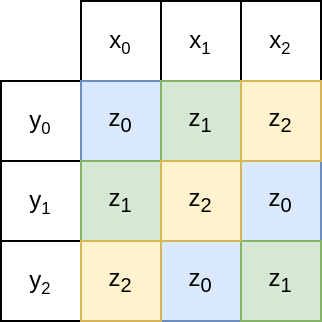
\includegraphics[width=\textwidth]{../resources/cyclic_convolution.drawio.png}
		\end{columns}
\end{frame}

\subsection{Acyclic convolution}

\begin{frame}
		\frametitle{\secname}
		\framesubtitle{\subsecname}

 		\begin{columns}
 				\column{0.5\textwidth}
				\textbf{Acyclic} convolution $u = x \times_A y$ is $2n$-length discrete
				signal with components:
				\note{Observe: Acyclic separates cylic into those where addition `wrapped around' vs those where it didn't}
				\begin{align*}
						u_k & \coloneqq \sum_{i + j = n} x_i \cdot y_j \\
						u_{2n - 1} & \coloneqq 0
				\end{align*}
 				\column{0.5\textwidth}
 				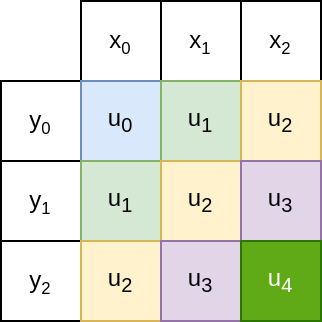
\includegraphics[width=\textwidth]{../resources/acyclic_convolution.drawio.png}
		\end{columns}
\end{frame}

\subsection{Negacyclic convolution}

\begin{frame}
		\frametitle{\secname}
		\framesubtitle{\subsecname}

 		\begin{columns}
 				\column{0.5\textwidth}
				\textbf{Negacyclic} convolution $v = x \times_\_ y$ is $n$-length discrete
				signal with components:
				\[
						v_k \coloneqq \sum_{i + j = n} x_i \cdot y_j - \sum_{i + j = n + k} x_i \cdot y_j
				\]
 				\column{0.5\textwidth}
 				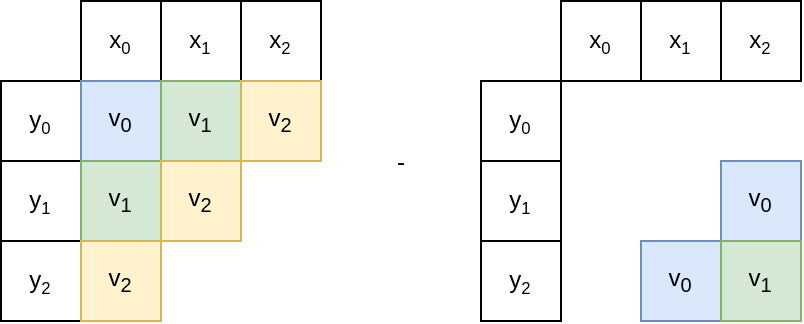
\includegraphics[width=\textwidth]{../resources/negacyclic_convolution.drawio.png}
		\end{columns}
\end{frame}

\subsection{Half-cyclic convolution}

\begin{frame}
		\frametitle{\secname}
		\framesubtitle{\subsecname}

 		\begin{columns}
 				\column{0.5\textwidth}
				\textbf{Half-cyclic} convolution $w = x \times_H y$ is $n$-length discrete
				signal with first $n$ components of acyclic convolution $x \times_A y$:
				\[
						w_k \coloneqq (x \times_A y)(k)
				\]
 				\column{0.5\textwidth}
 				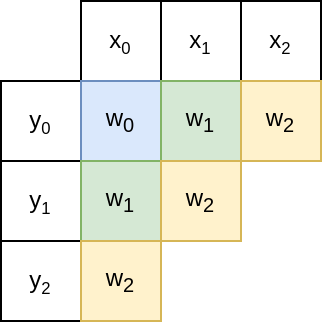
\includegraphics[width=\textwidth]{../resources/halfcyclic_convolution.drawio.png}
		\end{columns}
\end{frame}

\subsection{Relation between convolutions}

\begin{frame}
		\frametitle{\secname}
		\framesubtitle{\subsecname}

		Convolutions are related. Being able to e.g. calculate cyclic and
		negacyclic allows to also calculate half-cyclic or acyclic
		convolutions.

		\begin{align*}
				x \times_H y & = \frac{1}{2} \cdot ((x \times y) + (x \times_{\_} y)) \\
				x \times_A y & = (x \times_H y) || \frac{1}{2} \cdot ((x \times y) - (x \times_{\_} y)) \\
				L(x) \times_A L(y) & = x \times y = x \times_{\_} y
		\end{align*}
		\note{$L$ here is right-pad with zeros to length $2n$}
\end{frame}

\subsection{Convolution theorem}

\begin{frame}
		\frametitle{\secname}
		\framesubtitle{\subsecname}

		\note{Now we want to tie together convolutions and DFT}

		We can calculate the cyclic convolution using the DFT:
		\[
				x \times y = \DFT^{-1}(\DFT(x) \cdot \DFT(y))
		\]

		This is $O(n \log n)$ instead of the naive $O(n^2)$ if using the FFT.
\end{frame}

\subsection{Multiplication is a type of convolution!}

\begin{frame}
		\frametitle{\secname}
		\framesubtitle{\subsecname}

		\note{Why do we care about convolutions?}

		Consider long multiplication with a delayed carry operation.
		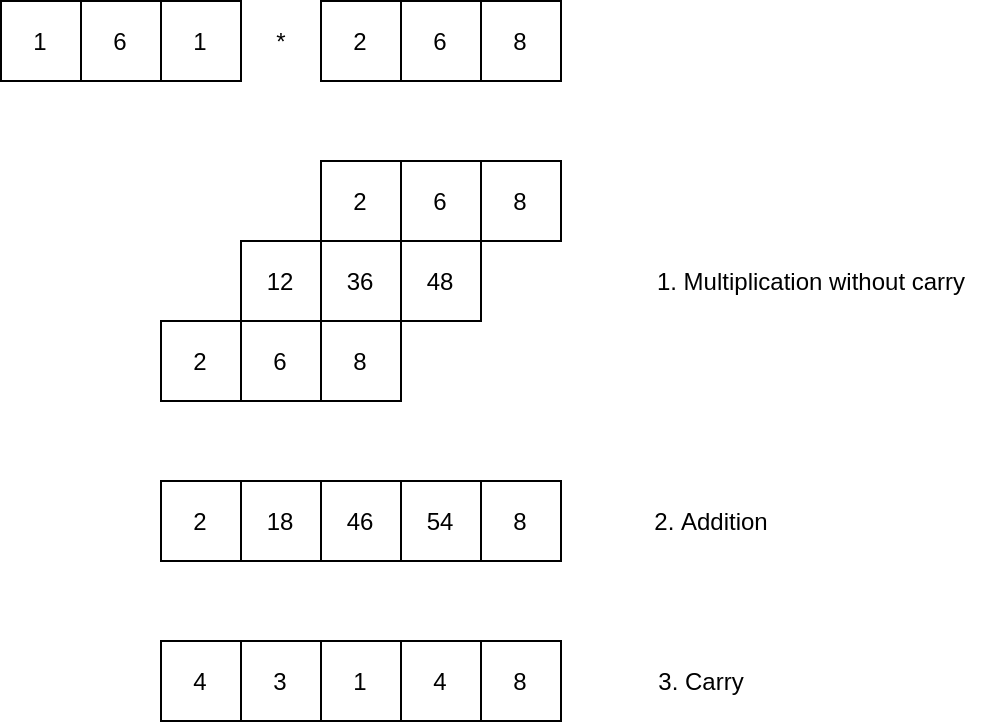
\includegraphics[width=0.7\textwidth]{../resources/long_multiplication.drawio.png}
\end{frame}

\begin{frame}
		\frametitle{\secname}
		\framesubtitle{\subsecname}

		The multiplication part is an acyclic convolution.
		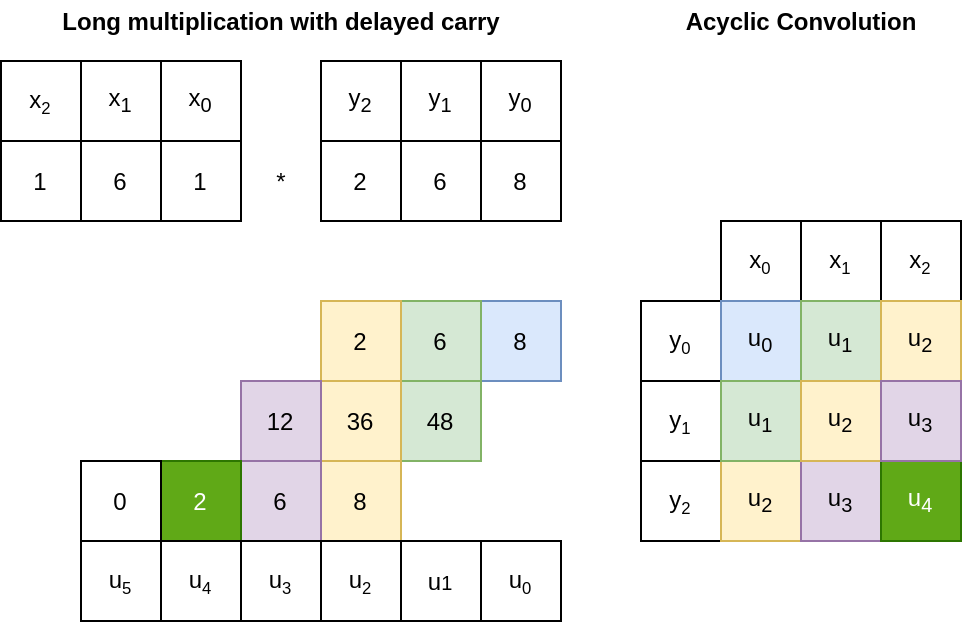
\includegraphics[width=0.7\textwidth]{../resources/multiplication_convolution.drawio.png}
\end{frame}

\section{FFT Multiplication}

\section{Schönhage-Strassen algorithm}

\section{Summary}

\begin{frame}
		\frametitle{References}
		\printbibliography
\end{frame}

% 
% \section{Discrete Fourier Transform}
% 
% \begin{frame}
% 		\frametitle{Discrete Fourier Transform (DFT)}
% 		\begin{itemize}
% 				\item Discrete signal $S = (s_0, s_1, \ldots, s_{n-1})$
% 						\begin{itemize}
% 								\item Physics / Mathematic POV: Finite
% 										evenly-spaced sample of a function
% 								\item Computer science POV: Sequence of
% 										elements. Digits, coefficients, ...
% 						\end{itemize}
% 				\item DFT of S can then be defined over different algebraic
% 						structures (complex field, finite fields, field of
% 						integers, ...)
% 				\item Where $g$ is a primitive $n$-th root of unity, and $k \equiv 0 \pmod{n}$
% 		\end{itemize}
% 
% 		\[
% 				\operatorname{DFT}(S) = \sum_{i=0}^{n-1} s_i \cdot g^{-i \cdot k}
% 		\]
% \end{frame}
% 
% 
% \section{Convolution theory}
% 
% \begin{frame}
% \end{frame}
% 
% \subsection{Cyclic convolution}
% 
% \begin{frame}
% \end{frame}
% 
% \subsection{Negacyclic convolution}
% 
% \begin{frame}
% \end{frame}
% 
% \subsection{Connection to multiplication}
% 
% \begin{frame}
% \end{frame}
% 
% \subsection{Convolution theorem}
% 
% \begin{frame}
% \end{frame}
% 
% 
% \section{Schönhage-Strassen algorithm}
% 
% \begin{frame}
% \end{frame}
% 
% \subsection{Performance}
% 
% \begin{frame}
% \end{frame}
% 
% \subsection{Viability}
% 
% \begin{frame}
% \end{frame}
% 
% 
% \section{Summary}
% 
% \begin{frame}
% \end{frame}


% \section{Background}
% 
% \subsection{Internet Computer}
% 
% \begin{frame}
% 		\frametitle{Internet Computer: Overview}
% 
% 		\begin{columns}
% 				\column{0.5\textwidth}
% 				\begin{itemize}
% 						\item Distributed general-purpose computer
% 								\note[item]{Distributed computer made out of multiple physical nodes}
% 						\item Byzantine fault tolerance
% 						\item Worked on by Swiss non-profit:
% 								\href{https://dfinity.org}{DFINITY}
% 								\note[item]{Based in Switzerland, research outposts in US}
% 						\item Runs `canisters': Code \& state
% 						\item Limitations
% 								\note[item]{Further elaborations on limitations later}
% 				\end{itemize}
% 				\column{0.5\textwidth}
% 				\includegraphics[width=\textwidth]{../resources/dfinity_ic}
% 				\\ \autocite{DfinitySodiumLaunch}
% 		\end{columns}
% 
% \end{frame}
% 
% \begin{frame}
% 		\frametitle{Internet Computer: Canister architecture}
% 		\begin{columns}
% 				\column{0.5\textwidth}
% 				\begin{itemize}
% 						\item Frontend and backend canisters
% 								\note[item]{Frontend: Serves static files.
% 										Allows use of any JS-based frontend frameworks,
% 								e.g. Angular}
% 								\note[item]{WASM: Open standard for binary executables,
% 										designed for high-performance applications within
% 								web browsers. Compilers for various languages exists.}
% 						\item Orthogonal persistence
% 								\note[item]{Orthogonal persistence: Memory
% 										persists between calls and updates. Different
% 										from classical cold-storage based architectures.
% 								Effects choice of data structures and algorithms.}
% 						\item Inter-canister-calls
% 								\note[item]{Asynchronous communication between
% 								canisters on network}
% 								\note[item]{Promotes splitting of app into
% 								individual parts, `microservices'}
% 								\note[item]{More details on function calls follow}
% 						\item Sharding
% 								\note[item]{Sharding: Memory limit of 4GB per canister requires
% 								sharding of data}
% 				\end{itemize}
% 				\column{0.5\textwidth}
% 				\includegraphics[width=\textwidth]{../resources/dfinity_canister}
% 		\end{columns}
% \end{frame}
% 
% \begin{frame}
% 		\frametitle{Internet Computer: Distributed computing}
% 		\note[item]{How to achieve fault tolerance?}
% 		\begin{columns}
% 				\column{0.5\textwidth}
% 				\begin{itemize}
% 						\item On-demand grouping of independent physical nodes
% 								into subnets
% 								\note[item]{On-demand grouping allows dynamic increase of
% 								processing power}
% 								\note[item]{Independent nodes ensures resilience towards
% 								outages and malicious data centre operators}
% 						\item Each canister runs within one subnet
% 						\item Eventually: Different types of subnets offering different levels
% 								of fault tolerance
% 								\note[item]{Subnet type affect number of nodes which may
% 								fail, thereby requiring minimum number of nodes per subnet}
% 				\end{itemize}
% 				\column{0.5\textwidth}
% 				\begin{figure}
% 						\includegraphics[width=\textwidth]{../resources/dfinity_subnets}
% 						\\ \autocite{DfinitySodiumLaunch}
% 				\end{figure}
% 		\end{columns}
% \end{frame}
% 
% \begin{frame}
% 		\frametitle{Internet Computer: Distributed computing}
% 		\begin{columns}
% 				\column{0.5\textwidth}
% 				\textbf{Update calls}
% 				\begin{itemize}
% 						\item Run on all machines in subnet
% 						\item Changes to memory persist
% 						\item Consensus
% 								\note[item]{Consensus ensures that memory of
% 										all nodes after execution is consistent, but
% 								must be achieved.}
% 						\item Slow (seconds)
% 				\end{itemize}
% 				\column{0.5\textwidth}
% 				\textbf{Query calls}
% 				\begin{itemize}
% 						\item Run on one machine in subnet only
% 								\note[item]{Query calls susceptible to faulty or malicious nodes}
% 						\item Changes to memory discarded
% 						\item Fast (milliseconds)
% 						\item[] % Empty bullet point to fix alignment of columns, as they are (vertically) centered. ;)
% 				\end{itemize}
% 		\end{columns}
% \end{frame}
% 
% \begin{frame}
% 		\note[item]{Various limitations hinted at during past slides, some of
% 		which will be elaborated upon.}
% 		\frametitle{Internet Computer: Limitations}
% 		\begin{itemize}
% 				\item Consensus
% 						\note[item]{IC approach to consensus: Deterministic
% 								execution. Allows leaderless system where majority of
% 						nodes wins.}
% 						\note[item]{Without determinism: Worst case each node
% 								has different memory after execution, impossible to
% 								find consensus while simultaneously being resistant to
% 						byzantine failures}
% 						\begin{itemize}
% 								\item IC: Deterministic execution
% 						\end{itemize}
% 				\item `Deterministic' randomness
% 						\begin{itemize}
% 								\item IC: Network-provided randomness
% 										\note[item]{Randomness: IC has a
% 												trusted network-wide source of
% 												randomness which may be queried. Result is
% 										deterministic for all nodes during a call.}
% 						\end{itemize}
% 				\item Networked IO
% 						\begin{itemize}
% 								\item Operations must be deterministic
% 								\item Operations must have no side-effects or
% 										be idempotent
% 										\note[item]{Networked IO: E.g. API call
% 												must not cause side-effects more than
% 										once, if called by all nodes}
% 										\note[item]{Neither determinisim nor idempotence guaranteed for arbitrary IO}
% 								\item Eventually: Network calls via Oracle
% 										\note[item]{But no support for network IO outside of IC currently}
% 						\end{itemize}
% 		\end{itemize}
% \end{frame}
% 
% 
% \subsection{Motoko}
% 
% \begin{frame}
% 		\frametitle{Motoko}
% 
% 		\begin{columns}
% 				\column{0.7\textwidth}
% 				\begin{itemize}
% 						\item Created for development on IC
% 						\item Actor-based programming: Intuitive approach to concurrency
% 								\note[item]{Actor: Entity which can send
% 										messages to other actors, and act on messages
% 								it received}
% 								\note[item]{Concurrency easy to model, as
% 								actors simply act on messages they receive}
% 						\item Type system: Static, supports generics,
% 								structural subtyping, checked pattern matching
% 								\note[item]{Static: Types known at compilation time}
% 								\note[item]{Generics: Doh}
% 								\note[item]{Structural: Equivalence of types
% 										based on whether, for each feature in a, a
% 										corresponding feature in b exists. See: Interfaces in Go}
% 								\note[item]{Pattern matching: Decomposition of
% 								structured data}
% 						\item Barebones stdlib
% 								\note[item]{Stdlib: Lacks time operations, hash
% 										functions, string encoding, network IO,
% 								randomness, ...}
% 				\end{itemize}
% 				\column{0.3\textwidth}
% 				\includegraphics[width=\textwidth]{../resources/motoko_logo}
% 		\end{columns}
% \end{frame}
% 
% \begin{frame}[fragile]
% 		\frametitle{Example application}
% 		\note[item]{Basic skeleton of a counting service}
% 		\begin{lstlisting}
% 				import Buffer "mo:base/Buffer";
% 		\end{lstlisting}
% 		\note[item]{Import components of stdlib}
% \end{frame}
% 
% \begin{frame}[fragile]
% 		\frametitle{Example application}
% 		\begin{lstlisting}
% 				actor Dracula {
% 				  var count : Nat = 0;
% 				  var historicalCounts : Buffer.Buffer<Nat> = Buffer.Buffer<Nat>(10);
% 		\end{lstlisting}
% 		\note[item]{Actor definition}
% 		\note[item]{Actor variables: Stable and regular}
% \end{frame}
% 
% \begin{frame}[fragile]
% 		\frametitle{Example application}
% 		\begin{lstlisting}
% 				  public func increment() : async () {
% 				    archive(count);
% 				    count += 1;
% 				  };
% 		
% 				  public func get() : async Nat {
% 				    return count;
% 				  };
% 		
% 				  public query func estimate() : async Nat {
% 				    return count;
% 				  };
% 
% 				  func archive(x : Nat) {
% 				    historicalCounts.add(x);
% 				  };
% 		\end{lstlisting}
% 		\note[item]{Update \& query func: No qualifier = update}
% 		\note[item]{Public \& local func}
% \end{frame}
% 
% \begin{frame}[fragile]
% 		\frametitle{Example application}
% 		\begin{lstlisting}
% 				  public func undo() : async () {
% 				    switch (historicalCounts.removeLast()) {
% 				      case (null) {
% 				        // No item left, cannot undo
% 				      };
% 				      case (?x) {
% 				        count := x;
% 				      };
% 				    };
% 				  };
% 				};
% 		\end{lstlisting}
% 		\note[item]{Update \& query func}
% 		\note[item]{Public \& local func}
% \end{frame}
% 
% 
% \subsection{Digital signatures}
% 
% \begin{frame}
% 		\frametitle{Digital signatures}
% 		\begin{itemize}
% 				\item Schemes, based on asymmetric cryptography, to ensure
% 						authentication and integrity of messages
% 						\begin{itemize}
% 								\item No confidentiality
% 										\note[item]{Comparable with hand-written signature \& wax seals}
% 						\end{itemize}
% 						\note[item]{Authentication: Identity of sender}
% 						\note[item]{Integrity: Message not modified in transit}
% 						\note[item]{Confidentiality: Message not readable by unauthorised entities}
% 				\item Used as part of fundamental standards, e.g. TLS or OpenPGP
% 						\note[item]{Hence affects nearly everything done on the
% 						internet. Mail, web browsing, VPNs, file transfer}
% 				\item Legal applications
% 				\item Multiple signature schemes based on underlying
% 						cryptographic primitives: RSA, DSA, ECDSA
% 		\end{itemize}
% \end{frame}
% 
% \subsection{RSA}
% 
% \begin{frame}
% 		\frametitle{RSA}
% 		\begin{itemize}
% 				\item Public-key cryptosystem based on difficulty of integer
% 						factorisation and RSA problem (e-th root modulo N)
% 						\note[item]{Based on difficulty of integer
% 								factorisation as knowledge of $p, q$ is
% 						sufficient to determine $d$ from $e$}
% 		\end{itemize}
% 		\begin{align*}
% 				\text{Given}\ p, q\ \text{prime},\ N := pq,\ \exists\ e, d: \\
% 				{(m^{e})}^{d} \equiv {(m^{d})}^{e} \equiv m \mod N
% 		\end{align*}
% 		\begin{itemize}
% 				\item $(N, e)$ as public key, $d$ as private key, given a message $m$
% 						\begin{itemize}
% 								\item Use as encryption scheme by computing ciphertext $c := m^e \mod N$
% 										\note[item]{Encryption: From which plaintext can be derived with private key}
% 								\item Use as signature scheme by computing signature $\sigma := m^d \mod N$
% 										\note[item]{Signature: From which message can be derived with public key}
% 						\end{itemize}
% 		\end{itemize}
% \end{frame}
% 
% 
% \section{RSA signatures on the Internet Computer}
% 
% \begin{frame}
% 		\note[item]{Now onto the main `meat' of the thesis: What was implemented}
% 		\frametitle{PKCS\#1 standard}
% 		\begin{columns}
% 				\column{0.75\textwidth}
% 				\begin{itemize}
% 						\item Open standard by RSA laboratories
% 						\item Specifies RSA-based encryption and signature schemes
% 								\note[item]{Focus on signature schemes, as it's what was implemented in Motoko}
% 						\item Signature schemes
% 								\note[item]{Signature scheme describes how to construct
% 										and verify signatures, e.g. how data must be
% 										hashed, padding scheme, what constitutes final
% 								signature etc}
% 								\note[item]{So-called schemes with appendix: Message not stored as part of signature}
% 						\item Used as part of e.g. X.509 PKI infrastructure
% 								\note[item]{X.509 then used by TLS}
% 								\note[item]{As such PKCS\#1 is comparably low-level standard}
% 						\item Implementations in e.g. OpenSSL, BouncyCastle
% 				\end{itemize}
% 				\column{0.25\textwidth}
% 				\begin{figure}
% 						\includegraphics[width=\textwidth]{../resources/pkcs1_usage}
% 				\end{figure}
% 		\end{columns}
% \end{frame}
% 
% 
% \begin{frame}
% 		\frametitle{RSASSA-PKCS1-v1\_5 deterministic signature scheme}
% 		\begin{columns}
% 				\column{0.5\textwidth}
% 				\begin{itemize}
% 						\item Deterministic
% 								\note[item]{Same message signed multiple times produces same signature always}
% 						\item Considered secure insofar as no attacks known,
% 								but standard advocates use of second scheme
% 						% \item Signature is self-contained, contains hash identifier
% 						\item \textbf{Note}: Confidentiality \& authenticity is
% 								ensured by subsequent RSA trapdoor function
% 				\end{itemize}
% 				\column{0.5\textwidth}
% 				\begin{figure}
% 						\includegraphics[width=\textwidth]{../resources/pkcs1_emsa_pkcs15}
% 						\note[item]{Algorithm: Hash message, prepend hash identifier, done}
% 				\end{figure}
% 		\end{columns}
% \end{frame}
% 
% 
% \begin{frame}
% 		\frametitle{RSASSA-PSS probabilistic signature scheme}
% 		\begin{columns}
% 				\column{0.5\textwidth}
% 				\begin{itemize}
% 						\item Probabilistic
% 						\item Provable security based on security of RSA 
% 								\note[item]{Provable security under some assumptions on utilised hash function}
% 								\note[item]{Provable secure meaning secure IFF RSA secure}
% 								\begin{itemize}
% 										\item In model where output of hash function truly uniform
% 												\note[item]{Random oracle model}
% 								\end{itemize}
% 						%\item No hash identifier contained in signature
% 						%		\note[item]{Used hash algorithm must be communicated separately from signature}
% 				\end{itemize}
% 				\column{0.5\textwidth}
% 				\begin{figure}
% 						\includegraphics[width=\textwidth]{../resources/pkcs1_emsa_pss}
% 						\note[item]{Algorithm: Go through steps}
% 						\note[item]{MGF1: Basically a more flexible (output can also be shorter) PRG}
% 				\end{figure}
% 		\end{columns}
% \end{frame}
% 
% \begin{frame}
% 		\frametitle{Motoko library}
% 
% 		Library supporting:
% 		\note[item]{Library was created to allow generation and verification of signatures. Supports:}
% 		\note[item]{As mentioned stdlib very barebones, so library has various utility methods}
% 
% 		\begin{itemize}
% 				\item RSA signatures based on PKCS\#1: Generation and
% 						verification of deterministic and probabilistic
% 						signatures
% 						\note[item]{Compatibility with standard ensures
% 								interoperability with other implementations based on
% 						standard, e.g. OpenSSL}
% 						\note[item]{Two examples follow}
% 				\item Utility methods: Base64 encoding, string encoding
% 						\note[item]{Base64: For interaction of library via CLI}
% 						\note[item]{String encoding: Only UTF-32 (Motoko limitation)}
% 				\item Big-number arithmetics
% 						\note[item]{Big-number arithmetics: Cost of naive
% 								modular exponentiation too high, basic optimized
% 						algorithms implemented instead}
% 				\item Heavily unit-tested, but not production-ready
% 						\note[item]{Then again, neither is the IC production-ready}
% 		\end{itemize}
% \end{frame}
% 
% 
% \begin{frame}[fragile]
% 		\frametitle{Motoko library: Generating signature}
% 		\note[item]{Motoko library to allow generation and verification of signatures}
% 		\note[item]{Example of how using the library for PSS signatures might look like}
% 		\note[item]{Library has no special support for key management, simply requires modulus and private / public exponent}
% 		\note[item]{Message as byte array: Eg encoded unicode sequence, binary file, ...}
% 		\begin{lstlisting}
% 				import RSA "RSA";
% 
% 				// privkey: Two primes & private RSA exponent
% 				let privkey = { p = ...; q = ...; d = ...; modulusBits = 1024; };    
% 
% 				// msg: Message as Byte array
% 				var msg : [Word8] = [0x00, ...];
% 				
% 				switch (RSA.pssSign(privkey, msg)) {
% 				  case (#ok(sig)) {
% 				    // sig: PSS signature as byte array
% 				  };    
% 				  case (#err(e)) {
% 				    // e: Error message as string
% 				  };    
% 				};    
% 		\end{lstlisting}
% \end{frame}
% 
% \begin{frame}[fragile]
% 		\frametitle{Motoko library: Verifying signature}
% 		\note[item]{Similar to generation. Note differences: Pubkey instead of
% 		privkey, and message and signature passed to verification}
% 		\begin{lstlisting}
% 				import RSA "RSA";
% 				
% 				// pubkey: Modulus & public RSA exponent
% 				let pubkey = { n = ...; e = ...; modulusBits = 1024; };
% 
% 				// msg & sig: Message and signature as byte arrays
% 				var msg : [Word8] = [0x00, ...];
% 				var sig : [Word8] = [0x00, ...];
% 				
% 				switch (RSA.pssVerify(pubkey, msg, sig, null)) {
% 				  case (#ok(Bool)) {
% 				    // True / false indicating whether signature valid
% 				  };
% 				  case (#err(e)) {
% 					// Signature verification failed
% 				  };
% 				};
% 		\end{lstlisting}
% \end{frame}
% 
% \begin{frame}
% 		\frametitle{Demo: Signing in Motoko, verifying in OpenSSL}
% 
% 		\begin{itemize}
% 				\item Local IC replica hosting demo application
% 				\item Allows signing and verifying
% 				\item Input and output in Base64
% 		\end{itemize}
% \end{frame}
% 
% % \section{Big-number arithmetic in Motoko}
% % 
% % \begin{frame}
% % 		\frametitle{Big-number arithmetic in Motoko}
% % 
% % 		\begin{alertblock}{Problem: Inefficiency of modular exponentiation}
% % 				Naive implementation: $m^d \mod N$ with $k$-bit exponents
% % 				requires $O(2^k)$ multiplications.
% % 				\note[item]{Hence naive implementation non-polynomial, so does
% % 				not scale reasonably with key length.}
% % 				\note[item]{Which ignores the non-negligible complexity of
% % 				multiplication itself}
% % 		\end{alertblock}
% % 
% % 		Three levels of optimization:
% % 		\begin{itemize}
% % 				\item Reduce exponent size: Chinese Remainder Theorem (CRT) \& Fermat's little theorem
% % 				\item Lower number of multiplications: Exponentiation by squaring
% % 				\item Improve speed of multiplication: Montgomery modular multiplication
% % 		\end{itemize}
% % \end{frame}
% % 
% % \begin{frame}
% % 		\frametitle{Reducing exponent size}
% % 
% % 		\note[item]{Not going into details, and leaving out certain complexities for briefness' sake}
% % 
% % 		\begin{block}{Fermat's little theorem}
% % 				Given $p$ prime:
% % 				\begin{align*}
% % 						a^{p - 1} \equiv 1 \mod p
% % 				\end{align*}
% % 		\end{block}
% % 		\note[item]{FLT: Allows `pulling out' multiples of prime $p$ from
% % 		exponent, for modular exponentiation modulo $p$}
% % 
% % 		\begin{block}{Chinese Remainder Theorem}
% % 				Goal: $m^d \mod N$, with $N = p \cdot q$, $p, q$ prime:
% % 				\begin{align*}
% % 						m_1 = m^{d \mod (p - 1)} \mod p \\
% % 						m_2 = m^{d \mod (q - 1)} \mod q \\
% % 						h = q_{inv} \cdot (m_1 - m_2) \mod p \\
% % 						q_{inv} \cdot q \equiv 1 \mod p \\
% % 						m^d \equiv m_2 + h \cdot q \mod N
% % 				\end{align*}
% % 		\end{block}
% % 		\note[item]{CRT: Allows turning exponentiation modulus $N$ into two
% % 		exponentiations modulus prime factors, which then allows applying FLT.}
% % \end{frame}
% % 
% % \begin{frame}
% % 		\frametitle{Exponentiation by squaring}
% % 
% % 		Given $a^b$, with $b_k, b_{k-1}, \ldots, b_1, b_0$ the binary representation of $b$, note that:
% % 		\begin{align*}
% % 				a^b = a^{\sum_{i=0}^{k} b_i \cdot 2^i} = \prod_{i=0}^{k} a^{b_i \cdot 2^i}
% % 		\end{align*}
% % 
% % 		\begin{itemize}
% % 				\item Each factor $a^{b_i \cdot 2^i}$ can be calculated by repeatedly squaring $a$
% % 				\item Iterate over bits of exponent, calculating the factors of the product along the way
% % 				\item Multiply result by factors where $b_i = 1$
% % 		\end{itemize}
% % \end{frame}
% 
% 
% \section{Summary}
% 
% \begin{frame}
% 		\frametitle{Summary}
% 
% 		\begin{itemize}
% 				\item Internet computer is decentralised, distributed,
% 						fault-tolerant computing platform
% 				\item A library to generate and verify RSA signatures based on
% 						the PKCS\#1 standard was created
% 				\item IC is an interesting concept, but far from ready for
% 						hosting real-life applications
% 						\note[item]{Missing crucial features such as IO}
% 				\item Motoko is a modern language with nifty features, but its stdlib is lacking
% 						\note[item]{To be expected from something this early}
% 				\item Lots of fun was had along the way
% 		\end{itemize}
% \end{frame}
% 
% 
% \section{Future work}
% 
% \begin{frame}
% 		\frametitle{Future work}
% 
% 		\begin{itemize}
% 				\item Implement PKCS\#1 encryption schemes
% 				\item Implement X.509 certificate management (generation, verification, ...)
% 				\item Further improve big-number arithmetic: Montgomery modular multiplication
% 		\end{itemize}
% \end{frame}
% 
% 
% \section{References}
% 
% \begin{frame}
% 		\frametitle{References}
% 		\printbibliography
% \end{frame}

\end{document}
